180. \begin{figure}[ht!]
\center{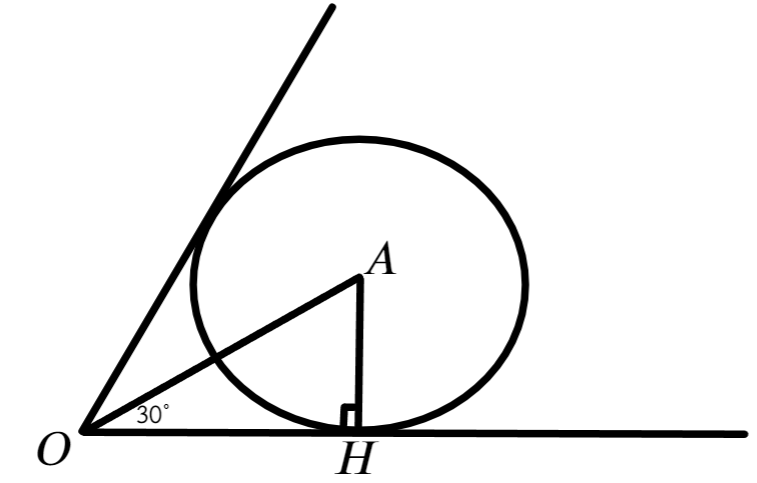
\includegraphics[scale=0.35]{g9-180.png}}
\end{figure}\\
Раз точка $A$ равноудалена от сторон угла, она лежит на его биссектрисе. Опустим перпендикуляр $AH,$ тогда $AH$ является радиусом окружности, и $\angle AOH=60^\circ:2=30^\circ.$ По теореме о катете, лежащем напротив угла в $30^\circ,$ имеем равенство $AH=OA:2=8:2=4,$ а длина окружности равна $2\pi\cdot4=8\pi.$
ewpage
oindent
